% !TEX root = main.tex

%------------------------------------------------
\chapter[Holomorphic Functions]{Differentiability and Holomorphic Functions}
\section{The Derivative of a Complex Function}
Throughout this section, let $U$ be an open subset of $\C$.  The definition of differentiability for a function $f: U \to \C$ looks almost identical to the corresponding definition for real functions.

\begin{definition}
Let $f: U \to \C$ be a function, and let $w \in U$.  We say that $f$ is \emph{differentiable at $w$} if the limit
\begin{equation}
\label{e:diff}
\lim_{\substack{z \to 0\\ z \in \C \backslash \set{0}}} \frac{f(w+z)-f(w)}{z}
\end{equation}
exists.  When it does, we denote its value by $f'(w)$.

%If $f$ is differentiable at $w$ for all $w \in U$, we say that $f$ is \emph{holomorphic on $U$}.
\end{definition}

Since $U$ is open, the quantity (the \emph{difference quotient})
\[
\frac{f(w+z)-f(w)}{z}
\]
is defined whenever $z$ is `sufficiently small' (to ensure that $w+z \in U$ and so $f(w+z)$ is defined) but not zero (to avoid division by zero). In other words, $0$ is a limit point of the domain of the difference quotient (regarded as a function of $z$).


\begin{wrapfigure}{l}{0.5\textwidth}
\begin{framed}
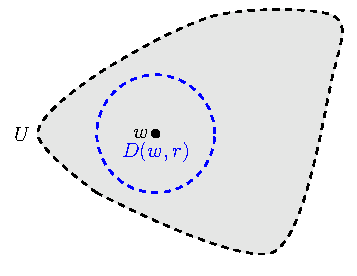
\includegraphics[scale=1]{holomorphicdomain}
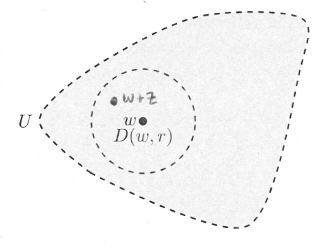
\includegraphics[scale=0.75]{openset_scan}
\caption{Since $U$ is open there is $r>0$ with $D(w,r) \subseteq U$.  For $0<\abs{z}<r$, $w+z$ lies inside this disc and hence the difference quotient is defined at $z$.}
\end{framed}
\end{wrapfigure}

 For this reason, we can again omit the second subscript and write~\eqref{e:diff} as
\[
\lim_{z \to 0} \frac{f(w+z)-f(w)}{z}
\]
without ambiguity.




\begin{example}
\label{e:diff1}
Let us investigate whether or not the function
\[
f:\C \to \C, \quad f(z)=-i\conj{z}
\]
is differentiable at any points $w \in \C$.
\end{example}

%1 page handwritten.
\begin{solution}
Fix $w \in \C$. To evaluate the limit
\[
\lim_{z \to 0} \frac{f(w+z)-f(w)}{z},
\]
we first try to simplify the expression
\[
\frac{f(w+z)-f(w)}{z}.
\]
For any $z \in \C \backslash \set{0}$, 
\[
\frac{f(w+z)-f(w)}{z} = \frac{-i\ \conj{(w+z)}-(-i)\conj{w}}{z} = -i \frac{\conj{z}}{z}.
\]
%\vspace*{8cm}
But then the limit
\[
\lim_{z \to 0} \frac{f(w+z)-f(w)}{z} = \lim_{z \to 0} -i \frac{\conj{z}}{z},
\]
is the same as the limit that we considered in Example~\ref{e:rlim}, except scaled by a factor of $-i$.  Hence this limit does not exist for the same reason; that is
\[
\rlim{z \to 0}{z \in \R \backslash \set{0}} -i \frac{\conj{z}}{z} = -i, \text{ while } \rlim{z \to 0}{z \in i\R \backslash \set{0}} -i \frac{\conj{z}}{z} = i.
\]
So $f$ is not differentiable at any point $w \in \C$.
\end{solution}



\begin{example}
\label{e:diff2}
The function $\mathbf{g}: \R^2 \to \R^2$ is defined by\marginpar{{\bf Note: } Both the real and the imaginary parts of $g$ are differentiable with respect to both $x$ and $y$ everywhere in $\R^2$.}
\[
\mathbf{g}(x,y)=(1,-x^2-y^2)\quad (x,y) \in \R^2.
\]
Find the corresponding complex function $g:\C \to \C$ and investigate where it is differentiable.
\end{example}

\begin{solution}
The corresponding function $g: \C \to \C$ is
\[
g(x+iy) = 1+i(-x^2-y^2),
\]
or equivalently,
\[
g(z) = 1-i z \conj{z}.
\]\marginpar{Since $x^2+y^2=\conj{z}z$}
Again, we fix $w \in \C$ and look at the difference quotient
\[
\frac{g(w+z)-g(w)}{z} = -i(w \frac{\conj{z}}{z}+\conj{w}+\conj{z})
\]
for $z \in \C \backslash \set{0}$.\\

As with the previous example, we have $\frac{\conj{z}}{z}$ appearing in the difference quotient, so it looks like our limit will not exist.  Again, we shall check by evaluating the restricted limits along the real and imaginary axes.

\begin{align*}
\rlim{z \to 0}{z \in \R \backslash \set{0}} -i \left( w \frac{\conj{z}}{z} + \conj{w} + \conj{z} \right) & = -i(w + \conj{w} ) \\
\rlim{z \to 0}{z \in i\R \backslash \set{0}} -i \left( w \frac{\conj{z}}{z} + \conj{w} + \conj{z} \right) & = -i (-w+\conj{w} ).
\end{align*}
These restricted limits are equal if and only if $w+\conj{w} = -w + \conj{w}$, which occurs if and only if $w=0$.  It follows that the unrestricted limit
\[
\lim_{z \to 0} \frac{g(w+z)-g(w)}{z}
\]
does not exist at any $w \in \C \backslash \set{0}$, hence $g$ is not differentiable at any of these points.

What about when $w=0$?  While the restricted limits along the real and imaginary axes are equal, this is \emph{not} enough to conclude that the unrestricted limit exists.  Indeed, we must verify this directly:
\[
\lim_{z \to 0} \frac{g(0+z)-g(0)}{z} = \lim_{z \to 0} -i \conj{z} = 0.
\]
\marginpar{Here we have used the fact that $z \mapsto \conj{z}$ is continuous (Example~\ref{e:cts}), and so limit can be found by substitution of $z=0$.}  In other words, $g$ is differentiable at $0$ (and nowhere else), with $g'(0)=0$.
%\vspace*{15cm}
\end{solution}




\begin{example}
\label{e:diff3}
Consider the function $f$ defined by $f(z)=\dfrac{1}{z}$.  At which points $w \in \C$ is $f$ differentiable?
\end{example}

\begin{solution}
Since the domain of $f$ is the (open) set $\C \backslash \set{0}$, we must necessarily restrict our attention to points $w$ in this set.  Then with $z \neq 0$, we have
\[
\frac{f(w+z)-f(w)}{z} = \frac{\left( \frac{1}{w+z} \right) - \frac{1}{w}}{z} = \frac{-1}{w(w+z)}.
\]
Since by assumption $w \neq 0$, the algebra of limits (Proposition~\ref{p:alglimits}) tells us that $-\dfrac{1}{w(w+z)} \to - \dfrac{1}{w^2}$ as $z \to 0$.  Thus $f$ is differentiable at every $w \in \C \backslash \set{0}$, with $f'(w) = -\dfrac{1}{w^2}$.
%\vspace*{6cm}
\end{solution}

\begin{example}
\label{e:diff4}
Fix $\alpha \in \C$ and let $f$ be the constant function $f(z) = \alpha$ for all $z \in \C$.  Then $f$ is differentiable at every point $w \in \C$, and satisfies $f'(w)=0$ for all $w \in \C$.
\end{example}
\begin{solution}
For any $w\in \C$, and $z \in \C \backslash \set{0}$,
\[
\frac{f(w+z)-f(w)}{z} = \frac{\alpha-\alpha}{z}=0 \to 0 \text{ as } z \to 0.
\]
\end{solution}

\begin{example}
If $f:U \to \C$ is differentiable at every point $w$ in $U$, and has $f'(w)=0$ for all $w$, is $f$ necessarily constant?
\end{example}

\begin{solution}
Not necessarily.  If $U=U_1 \cup U_2$ where $U_1$ and $U_2$ are disjoint open subsets of $\C$, and $f:U \to \C$ is defined by
\[
f(z) = \begin{cases}
0 & \text{ if } z \in U_1 \\
1& \text{ if } z \in U_2,
\end{cases}
\]
then $f'(z)$ exists and is equal to $0$ at every $z \in U$, but $f$ is non-constant.
\end{solution}
%\vspace*{5cm}

\begin{example}
\label{e:diff5}
Fix $\beta \in \C$ and let $f(z)=\beta z$.  Then $f'(w) = \beta$ for all $w \in \C$.
\end{example}

\begin{solution}
\[
\frac{f(w+z)-f(w)}{z} = \frac{\beta(w+z)-\beta w}{z}=\beta  \to 0 \text{ as } z \to 0.
\]
\end{solution}

\section{Holomorphic Functions}

\begin{definition}
Let $U \subseteq \C$ be an open set and $f:U \to \C$ a complex function.  If $f$ is differentiable at $w$ for all $w \in U$, we say that $f$ is \emph{holomorphic on $U$}.
\end{definition}
Why \emph{holomorphic} and not simply \emph{differentiable} on $U$?  One reason for this is that there are many functions $f$ that are differentiable on the real line, but fail to be differentiable throughout any open subset $U \subseteq \C$.


\begin{definition}
Let $f:U \to \C$ be a complex function and $w \in U$.  If there is some $r>0$ such that $f$ is differentiable at every point in the open disc $D(w,r)$, then $f$ is said to be \emph{holomorphic at $w$}.
\end{definition}

If a function $f$ is holomorphic at $w$, then it is differentiable at $w$, but the converse is not necessarily true.


\begin{example}
Let us examine whether or not the functions from Examples~\ref{e:diff1},~\ref{e:diff2} and~\ref{e:diff3} are holomorphic on any subsets of $\C$.

\begin{itemize}
\item $f(z)=-i\conj{z}$ is not differentiable at any $w \in \C$ and therefore not holomorphic on any $U \subseteq \C$.
%\vspace*{2cm}
\item $f(z) = 1-i z \conj{z}$ is differentiable at $0$ and nowhere else.  Since the one-point set $\set{0}$ is not an open set, there is no open subset $U \subseteq \C$ with $f$ holomorphic on $U$.
%\vspace*{3cm}
\item $f(z) = \dfrac{1}{z}$ is differentiable at every point of the (open) set $\C \backslash \set{0}$ and is therefore holomorphic on this set.
%\vspace*{3cm}
\end{itemize}

\end{example}




If $f:U \to \C$ is holomorphic on $U$, then we get a new function $f':U \to \C, \ z \mapsto f'(z)$, called the \emph{derivative of $f$}.  In other words, for $z \in U$, $f'(z)$ is defined as the limit
\[
f'(z) = \lim_{\substack{h \to 0 \\ h \in \C \backslash \set{0}}} \frac{f(z+h)-f(z)}{h}.
\]



As for differentiable functions in $\R$, we have sum, product, chain and quotient rules for holomorphic functions defined on open subsets of $\C$.

\begin{theorem}[Rules of Differentiation]
\label{t:diffrules}
Let $U$ and $V$ be open subsets of $\C$ and let $f:U \to \C$ and $g:V \to \C$ be holomorphic on $U$ and $V$ respectively.  Then
\begin{enumerate}
\item (Sum rule) $f+g$ is homomorphic on $U \cap V$ and $(f+g)'(z)=f'(z)+g'(z)$
\item (Scalar Multiples) For any $\alpha \in \C$, $(\alpha f )$ is holomorphic on $U$ and $(\alpha f)' (z) = \alpha f'(z)$
\item (Product Rule) $fg$ is holomorphic on $U \cap V$ and $(fg)'(z)=f'(z)g(z)+g'(z)f(z)$
\item (Quotient Rule) The quotient $f/g$ is holomorphic on $U \cap \set{ z \in V: g(z) \neq 0}$ and 
\[
\left( \frac{f}{g} \right) '(z) = \frac{f'(z)g(z)-f(z)g'(z)}{g(z)^2}
\]
\item (Chain Rule) $f \circ g$ is holomophic on $V \cap g^{-1}(U)$ and $(f\circ g)'(z) = f'(g(z))g'(z).$
\end{enumerate}
\end{theorem}

%\vspace*{7cm}
Since we only ever speak of a function being holomorphic on an \emph{open} subset $U \subseteq \C$, the statement of Theorem~\ref{t:diffrules} implicitly relies on the assumption that $U \cap V$, $U \cap \set{ z \in V: g(z) \neq 0 }$ and $V \cap g^{-1} (U)$ are all open whenever $U$ and $V$ are open and $f$ and $g$ are holomorphic.  These are all relatively easy to prove (the second and third rely on Proposition~\ref{p:diffimpliescontinuous}).

The proof of Theorem~\ref{t:diffrules} is very similar to that of the corresponding result for functions of a real variable, and is thus omitted.

\begin{example}
 Let $p:\C \to \C$ be a complex polynomial
\[
p(z) = \alpha_0 + \alpha_1z + \ldots + \alpha_n z^n.
\]
Then $p$ is holomorphic on $\C$.
\end{example}

\begin{solution}
We saw in Examples~\ref{e:diff4} and~\ref{e:diff5} that the functions $f(z) = \beta z$ and $g(z)= \alpha$ (where $\alpha, \beta \in \C$ are fixed), are holomorphic on $\C$ with derivatives $f'(z) = \beta$ and $g'(z)=0$ for all $z \in \C$.  Together with Theorem~\ref{t:diffrules}, this shows that $p(z)$ is holomorphic on $\C$ with derivative\marginpar{Thus complex polynomials can be differentiated using exactly the same rules as for real polynomials}
\[
p'(z) = \alpha_1 + 2\alpha_2 z + \ldots + n \alpha_n z^{n-1}.
\]
\end{solution}
\begin{note}
A similar argument shows that if $g(z) = \dfrac{1}{z^n}$ where $n >0$, then $g'(z) = -\dfrac{n}{z^{n+1}}$.
\end{note}

%\vspace*{6cm}


\begin{proposition}
\label{p:diffimpliescontinuous}
Let $f: U \to \C$ be differentiable at a point $w \in U$.  Then $f$ is continuous at $w$.
\end{proposition}

%\begin{proof}
%If $f$ is differentiable at $w$ then
%\[
%\lim_{\substack{h \to 0 \\ h \in \C \backslash \set{0}}} \frac{f(w+h)-f(w)}{h}
%\]
%exists and equals $f'(w)$.  Writing $z=w+h$, we have
%\[
%f'(w) = \lim_{ z \to w} \frac{f(z)-f(w)}{z-w}.
%\]
%Hence
%\begin{align*}
%\lim_{z \to w} \left[ f(z)-f(w) \right] &= \lim_{z \to w} \left[ \left( \frac{f(z)-f(w)}{z-w} \right) \left( z-w \right) \right] \\
%&= f'(w) \cdot 0 = 0,
%\end{align*}
%i.e., $\lim_{z \to w} f(z) = f(w)$.
%\end{proof}

\begin{example}
If $f$ is holomophic on $U$, is $f'$ holomorphic on $U$?\marginpar{In fact for holomorphic functions, the answer is yes.  This gives us an even stronger result: if $f:U \to \C$ is holomorphic on $U$, then $f$ is infinitely differentiable on $U$.  We shall return to this later on in the module.}
\end{example}
\begin{example}
In real analysis, consider $g:\R \to \R$ defined by
\[
g(x) = \begin{cases}
-x^2 & x<0 \\
x^2 & x\geq 0.
\end{cases}
\]
It is easily shown that $g$ is differentiable on $\R$ with $g'(x) = 2 \abs{x}$ for all $x \in \R$.  However, we know that $x \mapsto 2 \abs{x}$ fails to be differentiable at $0$.
\end{example}

%\vspace*{6cm}
\section{The Cauchy Riemann Equations}
Again, let $U \subseteq \C$ be open.  Suppose we are given $f:U \to \C$, then we have seen how to write $f$ as a sum of its real and imaginary parts:


\[ f(x+iy)=u(x,y)+iv(x,y) \]
for all $z=x+iy \in U$.  \

Written in terms of $z$, we have
\[
f(z) = \underbrace{\frac{f(z)+\conj{f(z)}}{2}}_{\text{Real}} + i \underbrace{\left(\frac{f(z)-\conj{f(z)}}{2i} \right)}_{\text{Real}}
\]



\begin{example}
If $u$ and $v$ are differentiable with respect to both $x$ and $y$, does it follow that $f$ is holomorphic?  
\end{example}

%\vspace*{2cm}
\begin{solution}
No.  We saw in Example~\ref{e:diff1} that
\[
f(x+iy) = 1-i (x^2+y^2),
\]
whose real and imaginary parts are differentiable everywhere in $\R^2$ with respect to both $x$ and $y$, is not differentiable at any point $w \in \C \backslash \set{0}$.
\end{solution}

For clarity, let us recall the definition of partial derivatives.



\begin{definition}
Suppose that $u: \R^2 \to \R$ is a function.  Then the \emph{partial derivatives} of $u$ with respect to $x$ and $y$ are the functions $\frac{\partial u}{\partial x}$ and $\frac{\partial u}{\partial y}$ respectively, defined via
\begin{align*}
\frac{\partial u}{\partial x} (x_0,y_0):&= \lim_{\substack{h\to 0\\h \in \R \backslash \set{0}}} \frac{u(x_0+h,y_0)-u(x_0,y_0)}{h}\\
\frac{\partial u}{\partial y} (x_0,y_0):&= \lim_{\substack{h\to 0\\h \in \R \backslash \set{0}}} \frac{u(x_0,y_0+h)-u(x_0,y_0)}{h}
\end{align*}
at the points $(x_0,y_0)$ where the limits exist.
\end{definition}

When $f=u+iv$, these partial derivatives look a bit like restricted limits of the limit that defines $f'(z)$ (or at least the real part of this limit).  Indeed, it is easy to show that
\[
\pd{u}{x} = \rlim{z \to 0}{ z \in \R \backslash \set{0} } \frac{\Re (f(w+z)) - \Re(f(w))}{z},
\]
but that
\[
\pd{u}{y} \neq \rlim{ z \to 0 }{z \in i \R \backslash \set{0} } \frac{\Re (f(w+z)) - \Re(f(w))}{z},
\]
as this time, the denominator is complex.




\begin{theorem}[Differentiability Implies the Cauchy-Riemann Equations]
\label{t:cr1}

Let $f$ be a complex-valued function defined on some open set $U$ and let $w=x_0+iy_0 \in U$.  Write
\[
f(x+iy) = u(x,y)+iv(x,y).
\]
Then if $f$ is differentiable at the point $w$ we have the following:

\begin{enumerate}
\item[(i)] The partial derivatives $\pd{u}{x}, \pd{u}{y}, \pd{v}{x}, \pd{v}{y}$ all exist at the point $(x_0,y_0) \in \R^2$ corresponding to $w$.
\item[(ii)] The partial derivatives satisfy the Cauchy-Riemann Equations at $(x_0,y_0)$:
\begin{equation}
\label{eq:cr}
\pd{u}{x} (x_0,y_0) = \pd{v}{y} (x_0,y_0),\quad \pd{u}{y} (x_0,y_0) = - \pd{v}{x} (x_0,y_0)
\end{equation}
\item[(iii)] At this point  the derivative of $f$ satisfies
\[
f'(w)= \pd{u}{x} (x_0,y_0) + i \pd{v}{x} (x_0,y_0) = \pd{v}{y} (x_0,y_0) - i \pd{u}{y} (x_0,y_0).
\]
\end{enumerate}
\end{theorem}

Before proving Theorem~\ref{t:cr1}, let us look at some examples that demonstrate how it is a powerful result.



\begin{example}
 Verify that the Cauchy-Riemann equations are satisfied by the function  $f(z)=z^2$.\\
\end{example}

Here we have
\[
f(x+iy) = \underbrace{x^2-y^2}_{u(x,y)} + i \underbrace{2xy}_{v(x,y)},
\]
and hence
\[
\pd{u}{x} = 2x = \pd{v}{y} \text{ and } \pd{u}{y} = -2y = - \pd{v}{x}.
\]
Thus~\eqref{eq:cr} holds at every $(x,y) \in \R^2$.  Moreover, we have
\[
\pd{u}{x} + i \pd{v}{x} = 2x+i2y = 2(x+iy) = 2z = f'(z),
\]
as expected.

\begin{example} 
Use the Cauchy-Riemann equations to investigate the differentiability of $f(z)=\conj{z}$.
\end{example}

This time
\[
f(x+iy) = \underbrace{x}_{u(x,y)} + i \underbrace{-y}_{v(x,y)},
\]
so that $\pd{u}{x} = 1$ while $\pd{v}{y}=-1$ and~\eqref{eq:cr} does not hold at any point $(x,y) \in \R^2$.\marginpar{Note that we need both of the equations in~\eqref{eq:cr} to hold.}
 Thus we conclude that $f(z) = \conj{z}$ is not differentiable at any point $ z \in \C$.

\begin{proof}%[Proof of Theorem~\ref{t:cr1}]
Since $f$ is differentiable at $w$ we know that
\[
\rlim{z\to 0}{z \in \C \backslash \set{0}} \frac{f(w+z)-f(w)}{z}
\]
exists and is equal to $f'(w)$.  In particular, all of corresponding restricted limits exist, and are also equal to $f'(w)$.  As before, we shall examine the restricted limits along the real and imaginary axes.

If we restrict $z$ to the nonzero real axis, then $z$ is of the form $z=h+0i$ for $h \in \R \backslash \set{0}$, and thus
\[
w+z = (x_0+h)+iy_0,
\]
which corresponds to the point $(x_0+h,y_0) \in \R^2$.  Thus the restricted limit satisfies:

%\vspace*{10cm}
\begin{align*}
f'(w) & = \rlim{h \to 0}{h \in \R \backslash \set{0}} \frac{f(w+h)-f(w)}{h} \\
& = \rlim{h \to 0}{h \in \R \backslash \set{0}} \frac{\left[ u(x_0+h,y_0)+iv(x_0+h,y_0) \right] - \left[ u(x_0,y_0)+iv(x_0,y_0) \right]}{h} \\
& \vspace*{2cm} \\
& = \left( \rlim{h \to 0}{h \in \R \backslash \set{0}} \frac{u(x_0+h,y_0)-u(x_0,y_0)}{h}  \right) +i \left(  \rlim{h \to 0}{h \in \R \backslash \set{0}} \frac{v(x_0+h,y_0)-v(x_0,y_0)}{h} \right)  \\
& = \pd{u}{x} (x_0,y_0)+i \pd{v}{x} (x_0,y_0).
\end{align*}

Hence both $\pd{u}{x}$ and $\pd{v}{x}$ exist at the point $(x_0,y_0)$, and the derivative of $f$ at $w$ satisfies
\begin{equation}
\label{eq:cr1}
\tag{$\dagger$}
f'(w) = f'(x_0+iy_0) = \pd{u}{x} (x_0,y_0)+i \pd{v}{x} (x_0,y_0).
\end{equation}
%\vspace*{7cm}

We shall now examine the restricted limit along the nonzero imaginary axis. This limit must also satisfy
\[
f'(w) = \rlim{z\to 0}{z \in i \R \backslash \set{0}} \frac{f(w+z)-f(w)}{z}.
\]
%\vspace*{3cm}
If $z \in i \R \backslash \set{0}$, then $z=0+ik$ for some $k \in \R \backslash \set{0}$, and so
\[
w+z=x_0+i(y_0+k),
\]
which corresponds to the point  $(x_0,y_0+k) \in \R^2$.

Thus
\begin{align*}
f'(w) & = \rlim{z \to 0}{z \in i\R \backslash \set{0}} \frac{f(w+z)-f(w)}{z} \\
& = \rlim{k \to 0}{k \in \R \backslash \set{0}} \frac{\left[ u(x_0,y_0+k)+iv(x_0,y_0+k) \right] - \left[ u(x_0,y_0)+iv(x_0,y_0) \right]}{ik} \\
& \vspace*{2cm} \\
& =   \rlim{k \to 0}{k \in \R \backslash \set{0}} \frac{i\ \left[ v(x_0,y_0+k)-v(x_0,y_0) \right]}{ik} +
 \rlim{k \to 0}{k \in \R \backslash \set{0}} \frac{u(x_0,y_0+k)-u(x_0,y_0)}{ik}     \\[5ex]
 & =   \rlim{k \to 0}{k \in \R \backslash \set{0}} \frac{v(x_0,y_0+k)-v(x_0,y_0)}{k} 
 -i \left( \rlim{k \to 0}{k \in \R \backslash \set{0}} \frac{u(x_0,y_0+k)-u(x_0,y_0)}{k} \right)     \\
 & = \pd{v}{y} (x_0,y_0)-i \pd{u}{y} (x_0,y_0).
\end{align*}
So $\pd{u}{y}$ and $\pd{v}{y}$ also exist at $(x_0,y_0)$, and the derivative of $f$ at $w$ also satisfies
\begin{equation}
\label{eq:cr2}
\tag{$\ddagger$}
f'(w) = f'(x_0+iy_0) = \pd{v}{y} (x_0,y_0) - i \pd{u}{y} (x_0,y_0).
\end{equation}
Equating the real and imaginary parts of the two expressions~\eqref{eq:cr1} and~\eqref{eq:cr2} for $f'(w)$ gives
\[
\pd{u}{x} (x_0,y_0) = \pd{v}{y} (x_0,y_0) \text{ and } \pd{v}{x}(x_0,y_0) = - \pd {u}{y} (x_0,y_0),
\]
which completes the proof.
%\vspace*{15cm}
\end{proof}

\section{Geometry of Derivatives for Complex-Valued Functions}
When working with differentiable functions in $\R$, it is useful to have the geometric picture of the derivative of a function $g: \R \to \R$ - for example, by considering $g'(x)$ as the slope of the tangent to the graph of $g$ at the point $(x,g(x))$.  In this section we will try to give a geometric description of the derivative of a holomorphic function $g:U \to \C$ at a point $w \in U$.  Since we cannot draw the graph of such a function, some care is needed.

Returning to the real case, consider the following graph of a function $g:\R \to \R$:
\begin{center}
%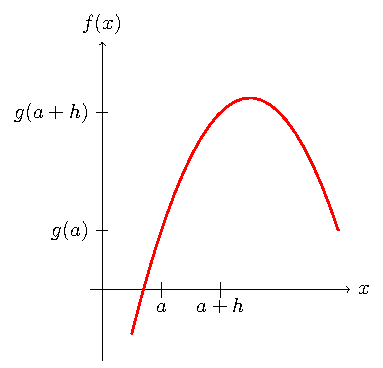
\includegraphics[scale=1]{realderivative1}
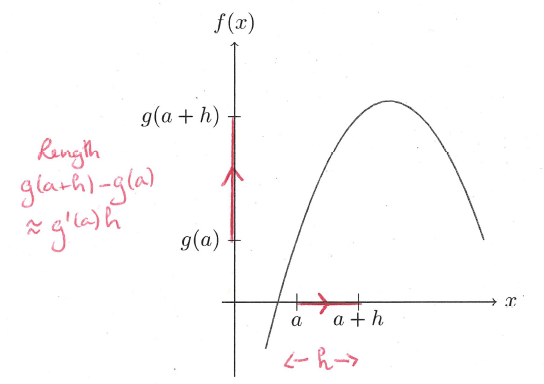
\includegraphics[scale=0.7]{derivative1_scan}
\end{center}

For sufficiently small $h$ we have
\[
\frac{g(a+h)-g(a)}{h} \approx g'(a),
\]
where $g'(a)$ is the value of the derivative of $g$ at $a$.  We can rewrite this approximation as
\[
g(a+h)-g(a) \approx g'(a) h.
\]
Now, we know that $g$ maps the interval $[a,a+h]$, of length $h$, to the interval $[g(a),g(a+h)]$ of length $g(a+h)-g(a)$  i.e. length approximately $g'(a)h$. 

In other words, $g$ moves $[a,a+h]$ to an interval from $g(a)$, and (approximately) scales it by a factor of $g'(a)$.
%\vspace*{3cm}

If $g'(a)$ is negative, then $[a,a+h]$ is approximately sent to $[g(a+h),g(a)]$. 
\begin{center}
%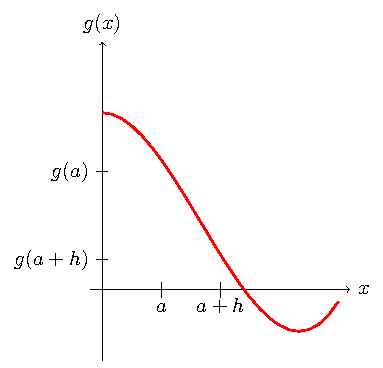
\includegraphics[scale=1]{realderivative}
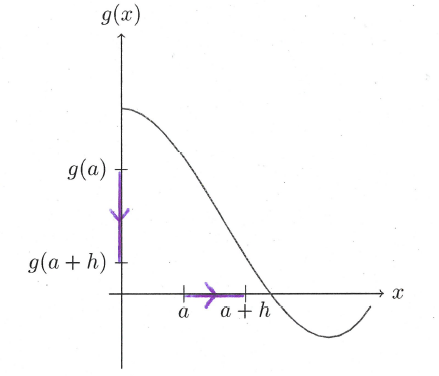
\includegraphics[scale=0.7]{derivative2_scan}
\end{center}
Then the mapping reverses the direction of the interval, i.e., sends $[a,a+h]$ to $[g(a+h),g(a)]$.  Again, the interval is scaled by a factor of $\abs{g'(a)}$, but this time, also rotated by an angle of $\pi$.  We can represent these mappings using one-dimensional figures as Figure~\ref{f:intervals} shows.

\begin{figure}[h]
\centering
%\vspace*{3cm}
%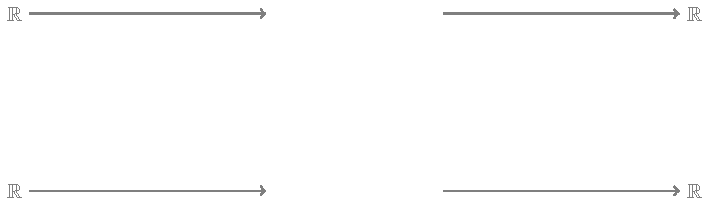
\includegraphics[scale=1]{4lines}
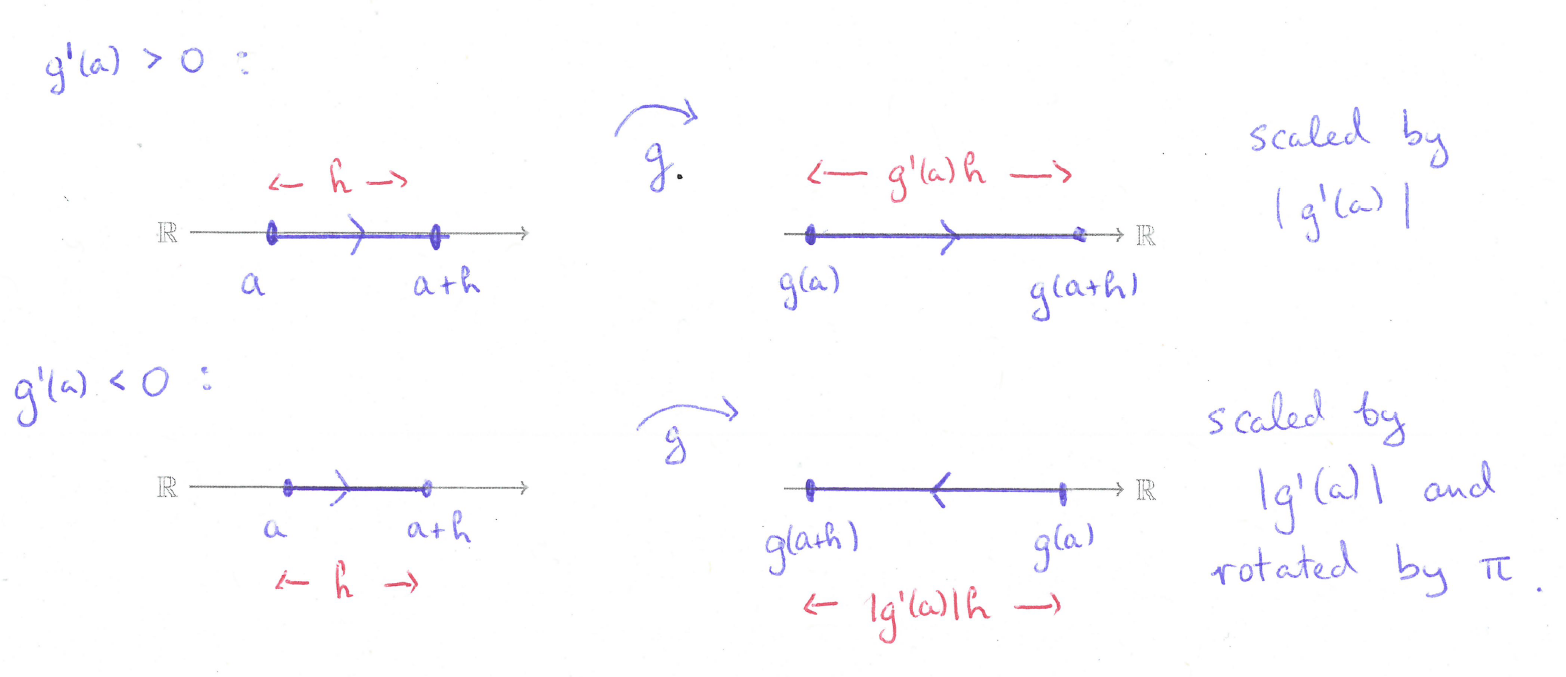
\includegraphics[scale=0.4]{4lines_full}
%\vspace*{3cm}
\caption{The image of a small interval $[a,a+h]$ under a function $g$.}
\label{f:intervals}
\end{figure}

For a complex function $f:U \to \C$, its graph is the set of points
\[
\set{ (z,f(z)): z \in U },
\]
as subset of $\C^2$.  We would need 4 coordinates to draw such a graph, which is impossible.

To describe the derivative of $f'(w)$ for a point $w \in U$, we will look at an analogy of Figure~\ref{f:intervals}.  Indeed, rather than looking at a small interval of the form $[a,a+h]$, we look at a small disk $D(w,r)$ centred at  $w$.

If $r$ is `small' and $z \in D(w,r)$ then
\[
\frac{f(w+z)-f(w)}{z} \approx f'(w),
\]
which can be rewritten as
\[
f(w+z) - f(w)\approx zf'(w).
\]
If we think of $z$ as the vector from $w$ to $w+z$, and $f(w+z)-f(w)$ as the vector from $f(w)$ to $f(w+z)$, then roughly speaking, $f$  sends $z$ to $zf'(w)$.  In other words, the vector $z$ gets moved to a vector from $f(w)$, and approximately gets multiplied by $f'(w)$, i.e.\marginpar{Again, we are using the fact that for $z_1,z_2 \in \C$, $\abs{z_1z_2} = \abs{z_1} \abs{z_2}$ and $\arg (z_1z_2) = \arg(z_1)+\arg(z_2)$.}
\begin{itemize}
\item scaled by a factor of $\abs{f'(w)}$ and
\item rotated by angle $\arg (f'(w))$ (about $f(w)$).
\end{itemize}
%\vspace*{5cm}
\begin{figure}[h]
%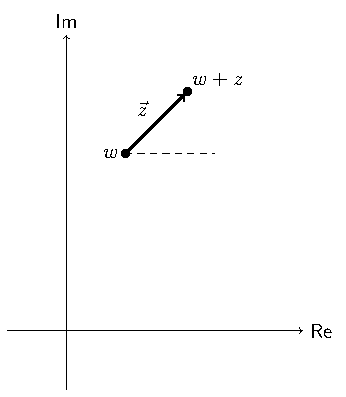
\includegraphics[scale=1]{deriv3} \qquad 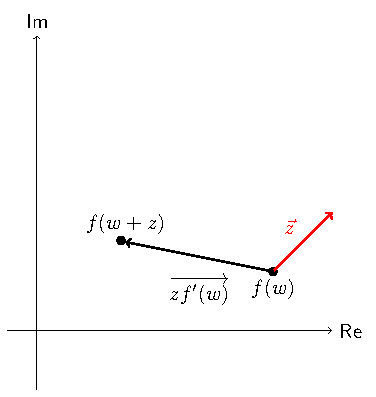
\includegraphics[scale=1]{deriv4}
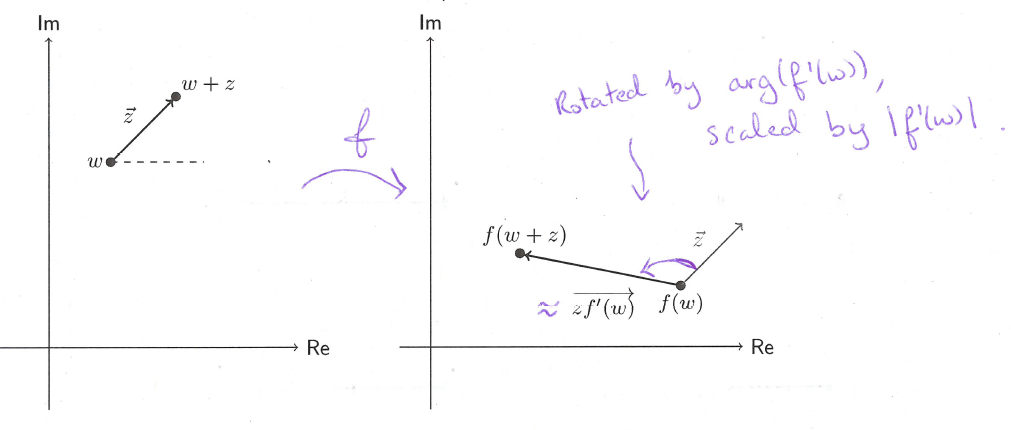
\includegraphics[scale=0.6]{deriv3_scan}
\caption{The effect of applying $f$ to points `near' $w$.  The vector $\vec{z}$ is sent to a vector from $w$, which is then scaled by $\abs{f'(w)}$ and rotated by $\arg (f'(w))$. In the diagram on the right, the angle between $\vec{z}$ and $\protect\overrightarrow{z f'(w)}$ is given by $\arg (f'(w))$.}
\end{figure}

The mapping $f$ transforms all points in $D(w,r)$ in the same way, thus
\begin{center}
\emph{$f$ maps small disks centred at $w$ to small disks centred at $f(w)$ as follows: scaling by a factor of $\abs{f'(w)}$ and rotating by angle $\arg (f'(w))$.}
\end{center}

\begin{figure}[h]
\centering
%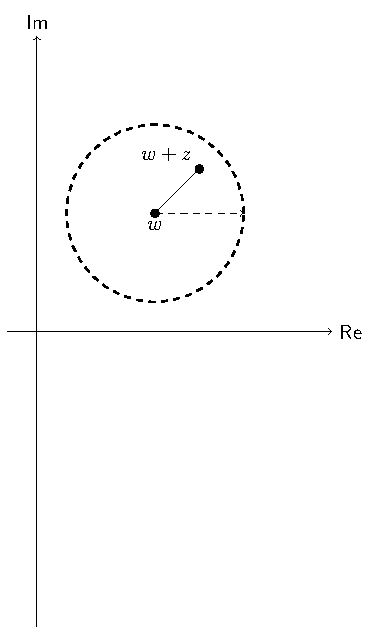
\includegraphics[scale=1]{derivative1}  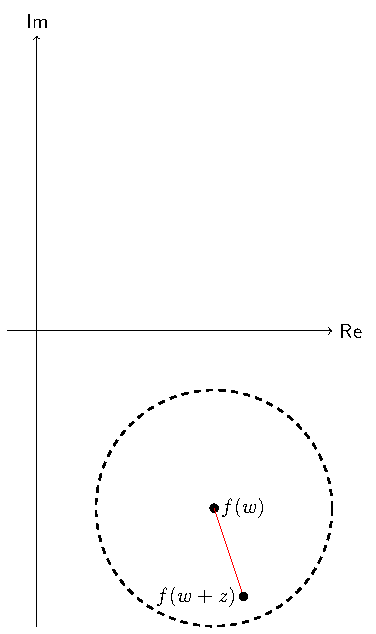
\includegraphics[scale=1]{derivative2}
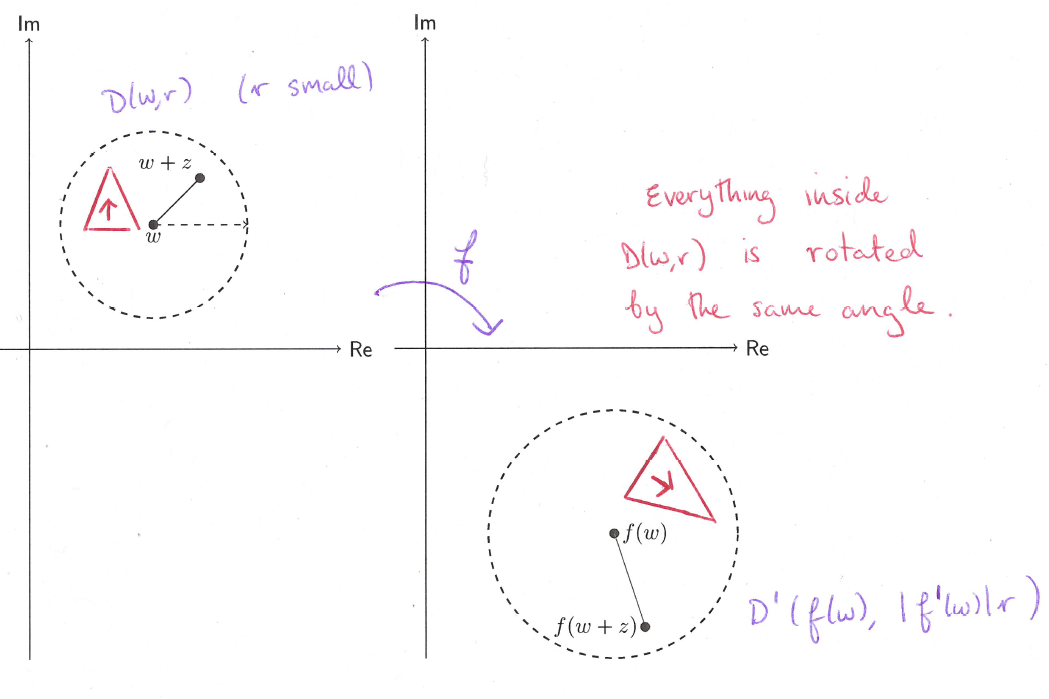
\includegraphics[scale=0.5]{deriv4_scan}
\caption{The image under $f$ of a small disc centred at $w$.}
\end{figure}

\begin{example}
Find the geometric effect of applying the function
\[
f(z)=z^2-\frac{i}{z^2}
\]
to a small disk centred at $i$.
\end{example}
%\vspace*{12cm}
Since $f$ is differentiable at $i$, the previous remarks indicate that a small disc centred at $i$ gets sent to a small disc centred at $f(i)$, where
\[
f(i) = i^2-\frac{i}{i^2} = -i+1.
\]
To determine the geometric effect of $f$ applied to this disc, we need to calculate $\abs{f'(i)}$ and $\arg (f'(i))$.  The rules of differentiation tell us that
\[
f'(z) = 2z-i \left( \frac{-2}{z^3} \right) = 2z+ \frac{2i}{z^3},
\]
and hence $f'(i) = 2i-2$, which has modulus $\abs{2i-2}=2\sqrt{2}$ and argument $3\pi/4$.

Hence a small disc at $i$ is approximately mapped to a small disc at $-1+i$, and is scaled by a factor of $2\sqrt{2}$ and rotated by an angle of $3\pi/4$  in the anticlockwise direction about $-1+i$.






\begin{figure}[h]
\centering
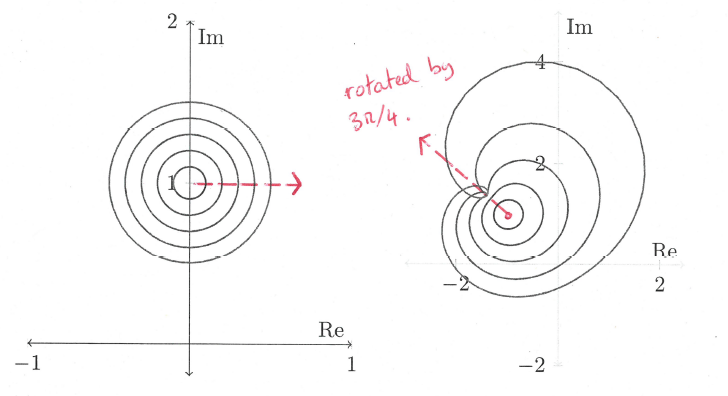
\includegraphics[scale=0.75]{parametric3_scan}
\caption{The geometric effect of applying $f(z)=z^2-\dfrac{i}{z^2}$ to small circles centred at $i$. The transformed circles are centred at $f(i)$.  As Figure~\ref{f:circles} shows, the images of the smaller circles are almost circular, but the larger ones less so.  The horizontal line from $i$ is rotated by $\arg(f'(w))$.}
\label{f:circles}
\end{figure}


\begin{example}
Find the geometric effect of applying the function $f$ defined via
\[
f(z)=\frac{z-i}{z+i}
\]
to a small disk centred at $i$.

\end{example}
%\vspace*{12cm}
This time, the disc gets mapped to a disc centred at $f(i) = \dfrac{i-i}{i+i} = 0$.  The quotient rule tells us that $f'(z) = \dfrac{2i}{(z+i)^2}$.  Hence $f'(i)=-i/2$ with modulus $1/2$ and argument $-\pi/2$.

In other words, a small disc centred at $i$ is mapped to a small disc centred at $0$, and is scaled by a factor of $1/2$ and rotated by an angle of $\pi/2$ \emph{clockwise} (since this time the argument of $f'(i)$ is negative) about $0$.

\begin{figure}[h]
\centering
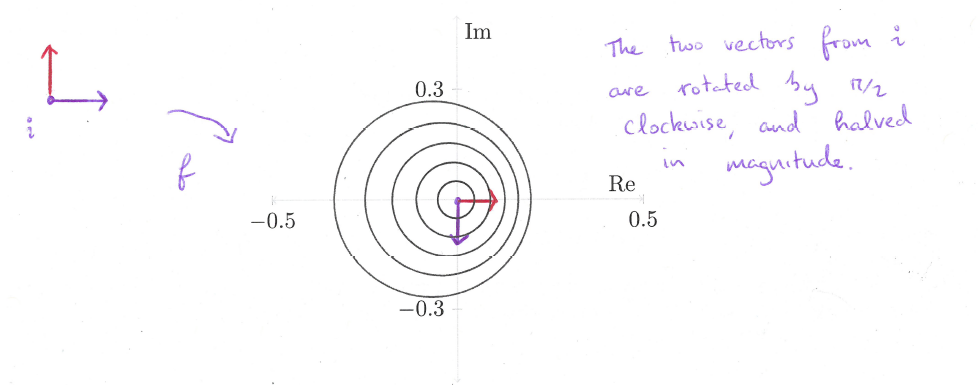
\includegraphics[scale=0.625]{parametric5_scan}
\caption{The images of circles centred at $i$ under the map $f(z)=\dfrac{z-i}{z+i}$}
\end{figure}
